\documentclass[a4paper,12pt]{report}
\usepackage{ctex}
\usepackage{color}
\usepackage{graphicx}
\usepackage{caption}
\usepackage{listings}   
\usepackage{hyperref}
\usepackage{verbatim}
\begin{document}
\title{系统开发工具基础}
\author{肖扬\\计算机科学与技术\\
学号：25020007140}
\date{2026年8月24日}
\maketitle

\pagenumbering{roman}
\tableofcontents
\newpage
\pagenumbering{arabic}

\color{red}\chapter{实验环境说明}
\color{black}
\begin{enumerate}
    \item {\large 系统版本：Ubuntu 22.04.1 LTS，用户名 xy\_ai，WSL2 架构}
    \item {\large 编译器：gcc 11.4.0、GNU Make 4.3（都在 /usr/bin）}
    \item {\large shell:bash 5.1.16（x86\_64-pc-linux-gnu）}
    \item {\large git: 2.34.1（Ubuntu 22.04 官方源版本，系统级）}
    \item {\large LaTeX:TeX Live 2022/dev（Debian 版），含xelatex、pdflatex、latexmk}
    \item {\large 所有任务均在base这个环境中进行，没有使用其他环境}
\end{enumerate}

\color{red}\chapter{课堂学习部分}
\color{black}
\section{第 1 题 含空格文件名的批量整理}
\begin{center}
    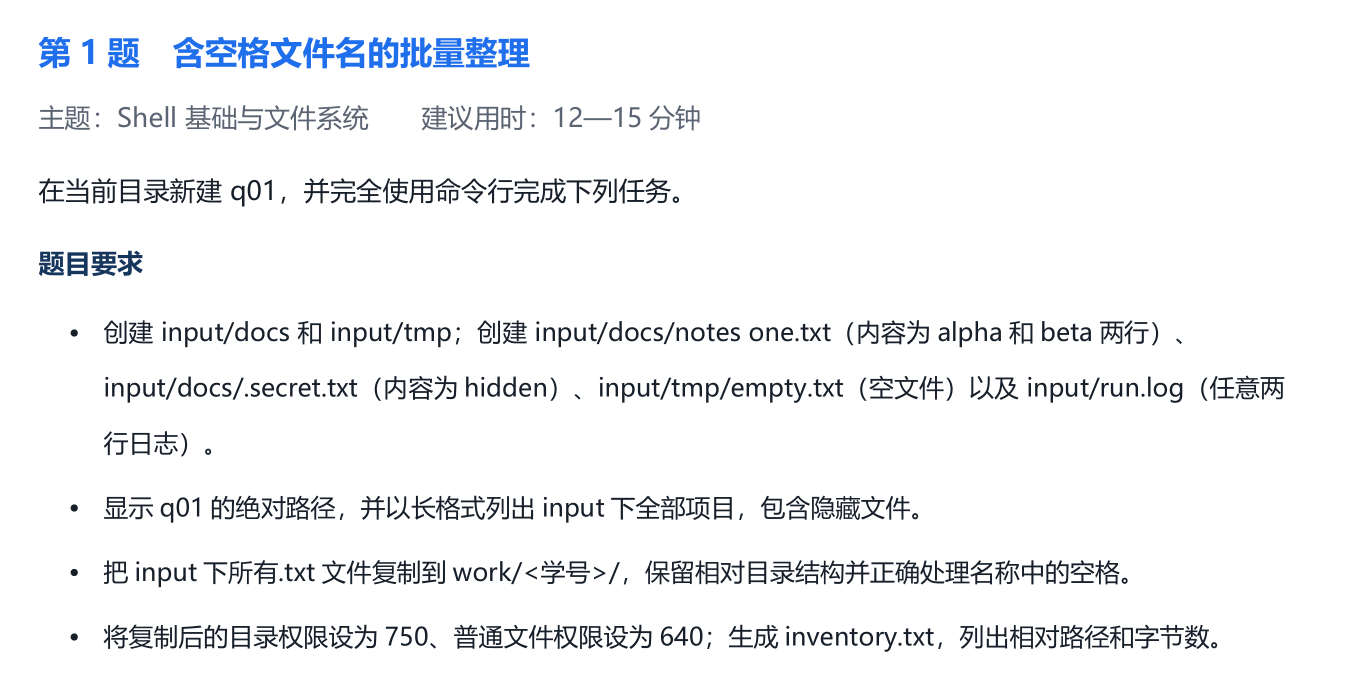
\includegraphics[width=0.88\textwidth]{13.png}
\end{center}
\begin{enumerate}
    \item {\large 确定当前路径，查看文件创建前目录}
    \begin{center}
        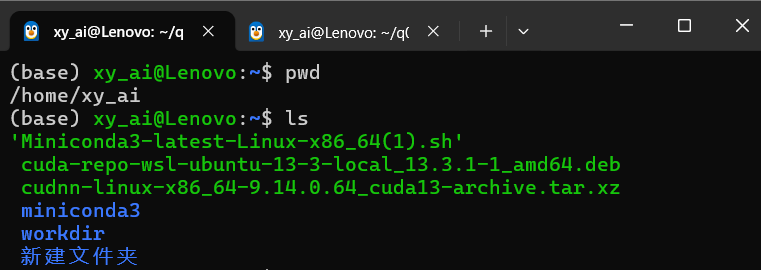
\includegraphics[width=0.88\textwidth]{photo3.png}
        \captionof{figure}{}
    \end{center}
    \item {\large 建立q01并验证}
    \begin{center}
        
\includegraphics{photo4.png}
        \captionof{figure}{}
        \par\vspace{4pt}
        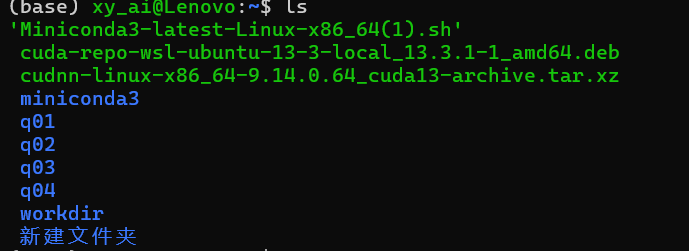
\includegraphics[width=0.84\textwidth]{check_the_four_document.png}
        \captionof{figure}{图为完成四项实验之后的截图}
    \end{center}
    \item {\large 创建 input/docs 和 input/tmp并验证}
    \begin{center}                                                                                                     
        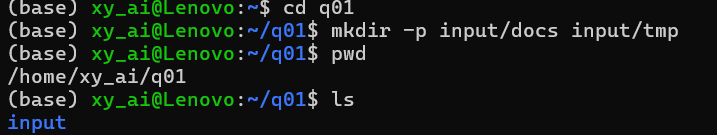
\includegraphics[width=0.84\textwidth]{photo5.png}
        \captionof{figure}{}
        \par\vspace{4pt}
        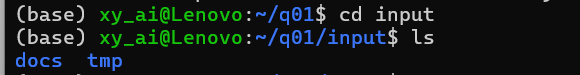
\includegraphics[width=0.84\textwidth]{photo6.png}
        \captionof{figure}{}
    \end{center}
    \item {\large 创建 input/docs/notes one.txt（内容为 alpha 和 beta 两行）、
input/docs/.secret.txt（内容为 hidden）、input/tmp/empty.txt（空文件）以及 input/run.log（任意两
行日志）}
    \begin{center}
        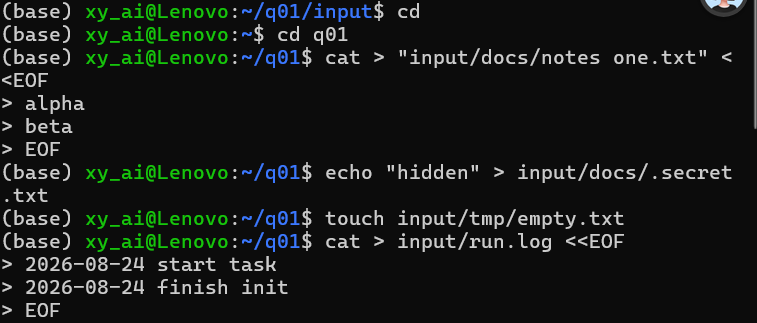
\includegraphics[width=0.88\textwidth]{photo7.png}
        \captionof{figure}{}
    \end{center}
    \item {\large 显示 q01 的绝对路径，并以长格式列出 input 下全部项目，包含隐藏文件}
    \begin{center}
        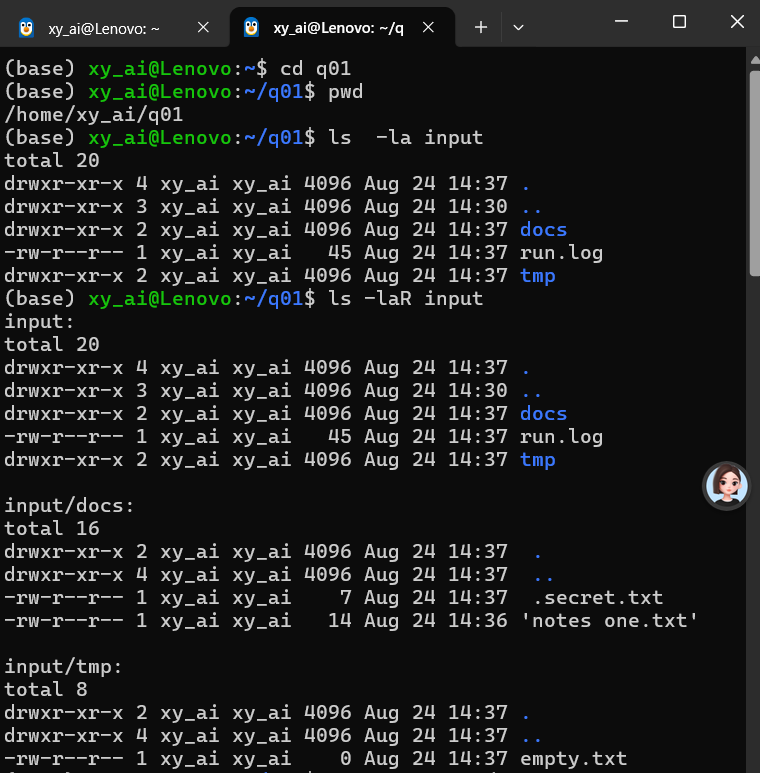
\includegraphics[width=0.88\textwidth]{photo8.png}
        \captionof{figure}{ls -la input不会进入 docs、tmp 子目录，不符合题目要求，所以使用ls -laR input}
    \end{center}
    \item {\large 把 input 下所有.txt 文件复制到 work/<学号>/，保留相对目录结构并正确处理名称中的空格}
    \begin{center}
        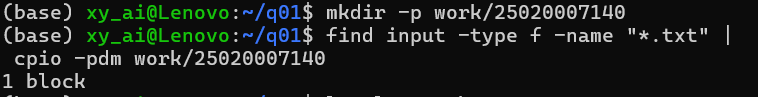
\includegraphics[width=0.88\textwidth]{9.png}
        \captionof{figure}{}
    \end{center}
    \noindent 第二段代码说明：
    \begin{itemize}
        \item find input：在 input 文件夹（及其所有子目录）中查找。
        \item -type f：只找普通文件（忽略目录）。
        \item -name "*.txt"：只找文件名以 .txt 结尾的文件。
        \item |（管道符）：将前半部分 find 查到的文件路径列表，直接传给后面的 cpio 命令处理。
        \item cpio：这是一个归档/复制工具（比 cp 更强）。
        \item-p（pass-mode，传递模式）：告诉 cpio 不要打包，而是直接复制文件到指定目录。
        \item -d（make directories）：在目标目录中自动创建子目录。也就是说，如果源文件在 input/docs/ 下，目标位置也会自动建一个 docs/ 文件夹。
        \item -m（preserve modification time）：复制时保留文件原有的修改时间（不改成当前时间）。
        \item work/25020007140：最终的目标根目录。
    \end{itemize}
    \item {\large 将复制后的目录权限设为 750、普通文件权限设为 640}
    \begin{center}
        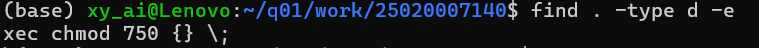
\includegraphics[width=0.88\textwidth]{10.png}
        \captionof{figure}{}
        \par\vspace{4pt}
        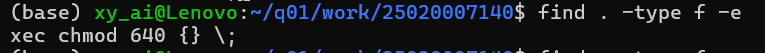
\includegraphics[width=0.85\textwidth]{11.png}
        \captionof{figure}{}
        \par\vspace{4pt}
        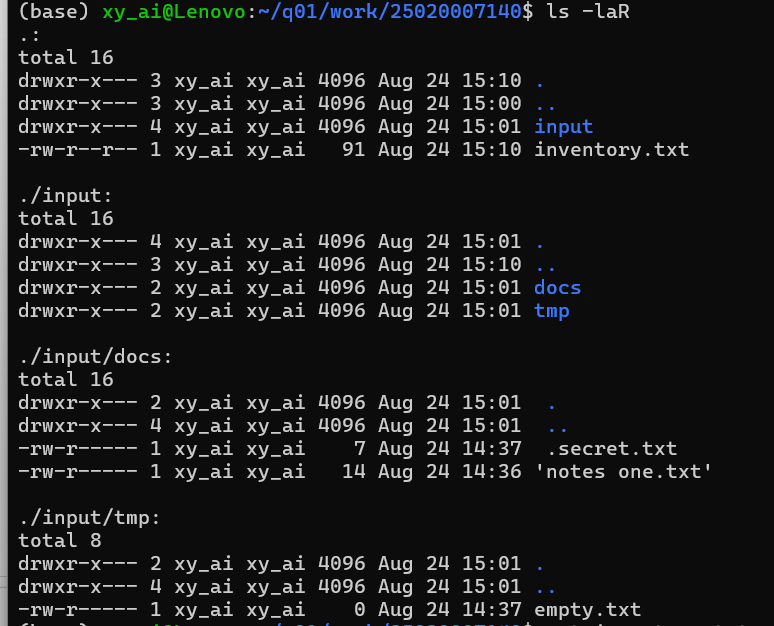
\includegraphics[width=0.85\textwidth]{14.png}
        \captionof{figure}{所有文件夹：rwxr-x--- = 750,普通文本文件：‑rw‑r----- = 640}
    \end{center}
    \item {\large 生成 inventory.txt，列出相对路径和字节数}
    \begin{center}
        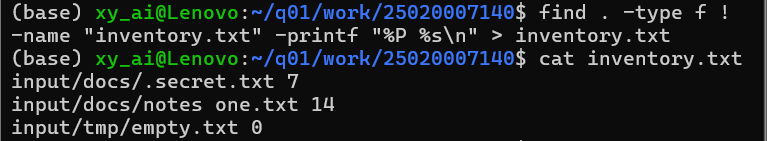
\includegraphics[width=0.88\textwidth]{12.png}
        \captionof{figure}{}
    \end{center}
\end{enumerate}
\section{第 2 题 随机访问日志统计}
\begin{center}
    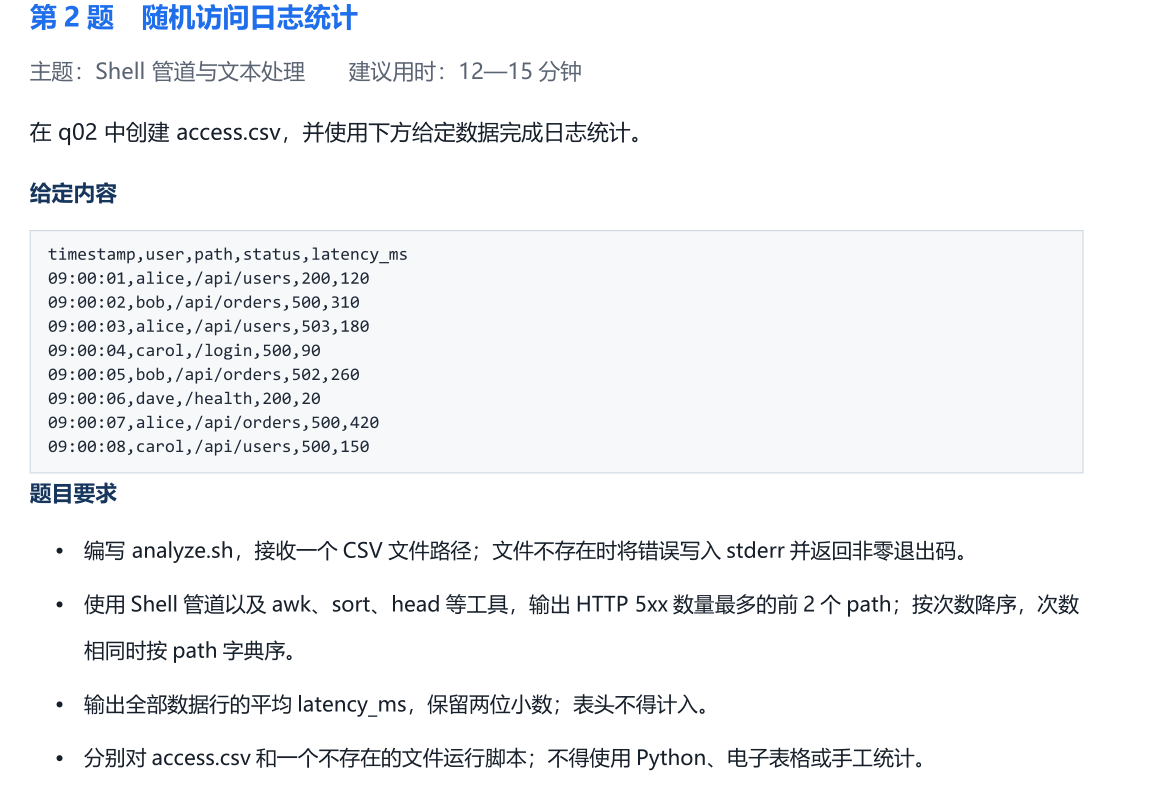
\includegraphics[width=0.88\textwidth]{15.png}
\end{center}
\begin{enumerate}
    \item {\large 创建 q02 目录，进入 q02。创建 access.csv，写入题目给的 CSV 数据，并验证数据数据是否正确}
    \begin{center}
        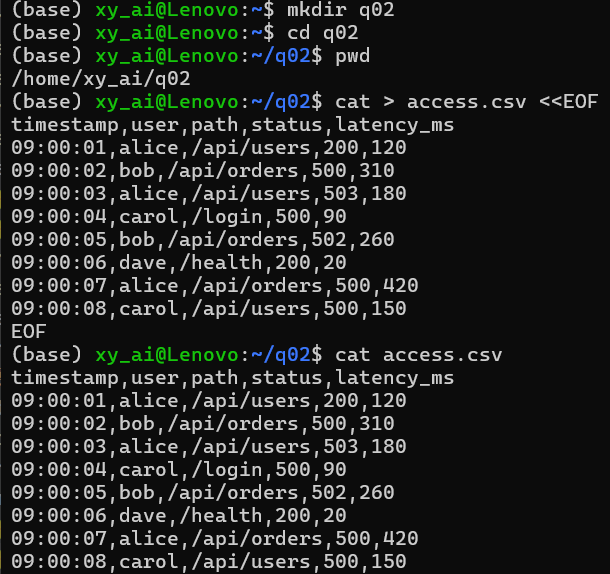
\includegraphics[width=0.88\textwidth]{16.png}
        \captionof{figure}{}
    \end{center}
    \item {\large 新建 analyze.sh，注意第二张图片analyse的截图只供第一小问使用，这是当时截图。后面截图会反映文件的修改，这是为了更好说明解题思路。}
    \begin{center}
        
\includegraphics[width=0.88\textwidth]{17.png}
        \par\vspace{4pt}
        \captionof{figure}{}
        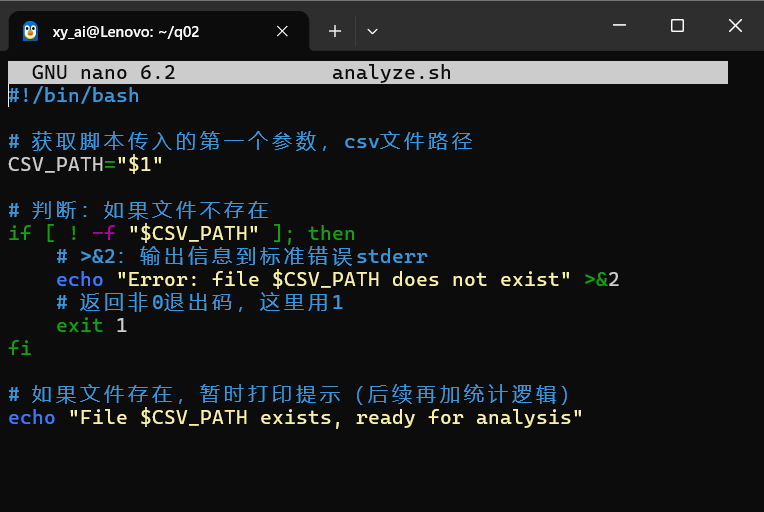
\includegraphics[width=0.88\textwidth]{18.png}
        \captionof{figure}{仅供第一问使用}
    \end{center}
    \item {\large 给脚本增加可执行权限}
    \begin{center}
        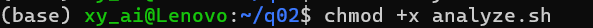
\includegraphics[width=0.88\textwidth]{19.png}
        \captionof{figure}{否则报错Permission denied}
    \end{center}
    \item {\large 文件不存在时将错误写入 stderr 并返回非零退出码}
    \begin{center}
        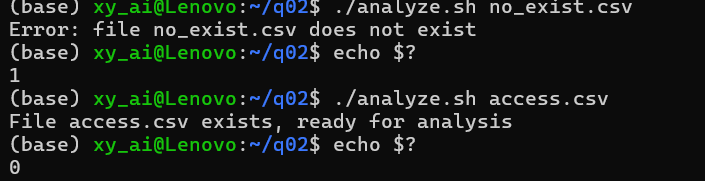
\includegraphics[width=0.88\textwidth]{20.png}
        \captionof{figure}{}
    \end{center}
    \item {\large 使用 Shell 管道以及 awk、sort、head 等工具，输出 HTTP 5xx 数量最多的前 2 个 path；按次数降序，次数
相同时按 path 字典序}
    \begin{center}
        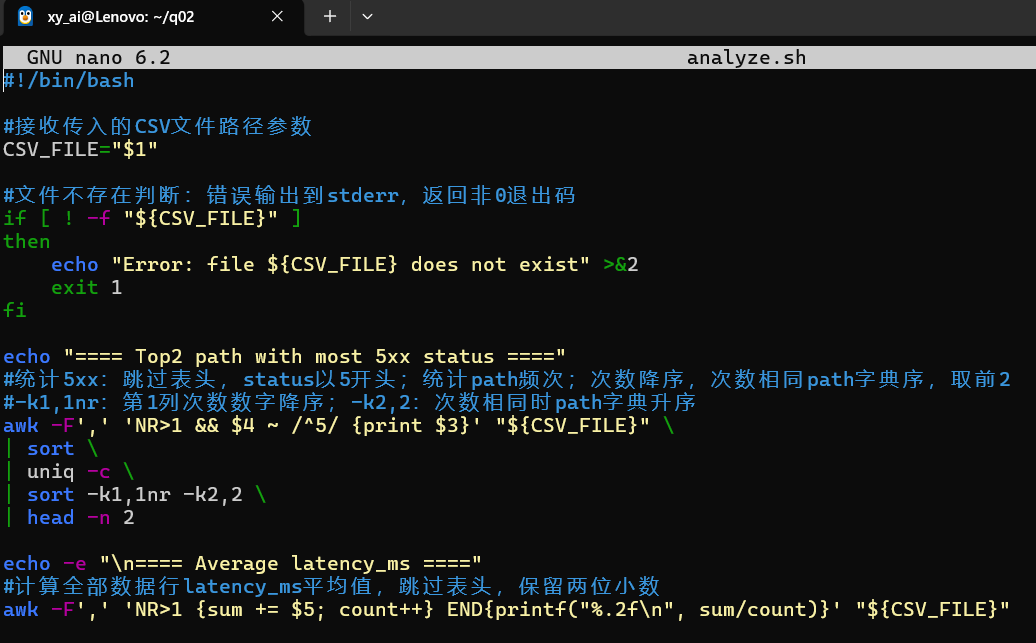
\includegraphics[width=0.88\textwidth]{21.png}
        \captionof{figure}{}
    \end{center}
    \item {\large 给脚本增加可执行权限}
    \begin{center}
        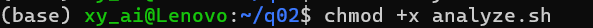
\includegraphics[width=0.88\textwidth]{19.png}
        \captionof{figure}{否则报错Permission denied}
    \end{center}
    \item {\large 输出全部数据行的平均 latency\_ms，保留两位小数；表头不得计入。}
    \begin{center}
        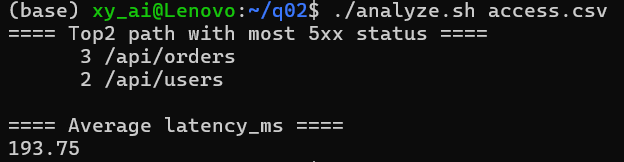
\includegraphics[width=0.88\textwidth]{22.png}
        \captionof{figure}{}
    \end{center}
    \item {\large 分别对 access.csv 和一个不存在的文件运行脚本；不得使用 Python、电子表格或手工统计}
    \begin{center}
        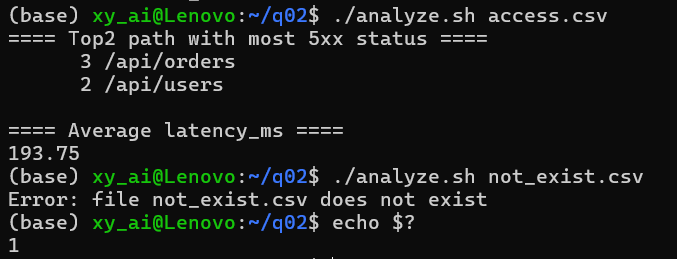
\includegraphics[width=0.88\textwidth]{23.png}
        \captionof{figure}{}
    \end{center}
    
\end{enumerate}



\section{第 3 题 制造、解决并解释一次合并冲突}
\begin{center}
    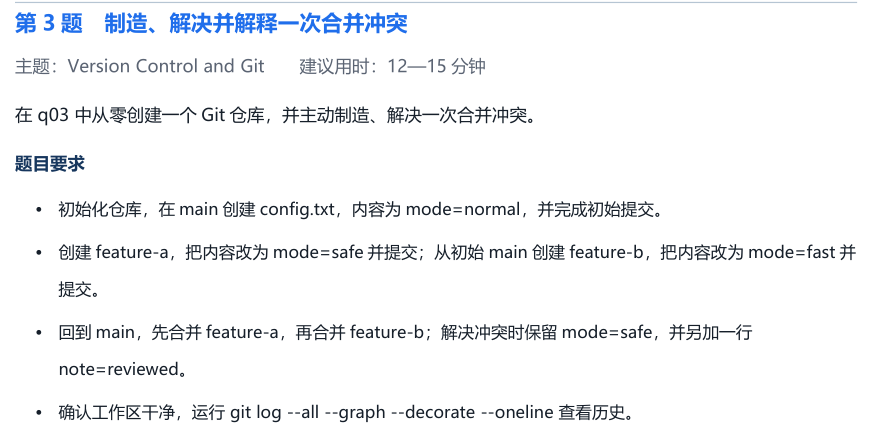
\includegraphics[width=0.85\textwidth]{34.png}
    \captionof{figure}{题目信息}
\end{center}
\begin{enumerate}
    \item {\large 创建q03并进入初始化仓库，将分支改名为main}
    \begin{center}
        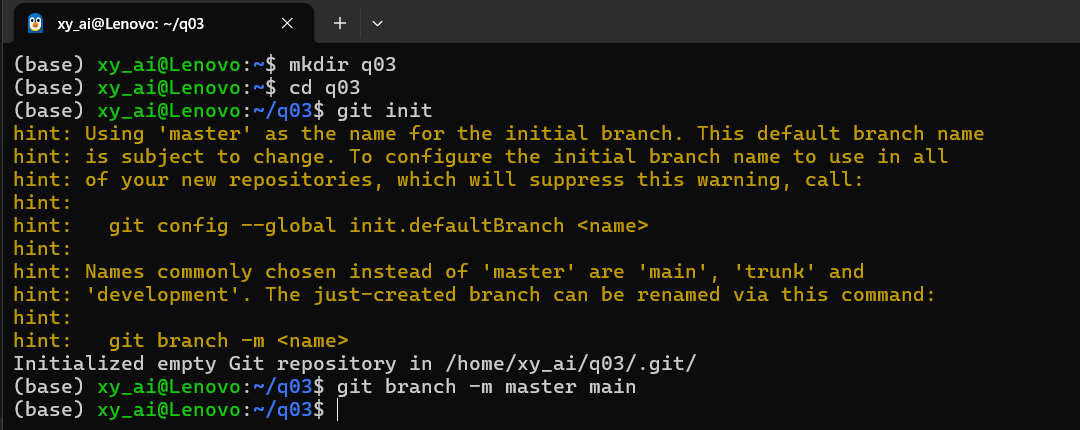
\includegraphics[width=0.85\textwidth]{35.png}
        \captionof{figure}{}
    \end{center}
    \item{\large main 分支初始提交，创建 config.txt，内容mode=normal}
    \begin{center}
        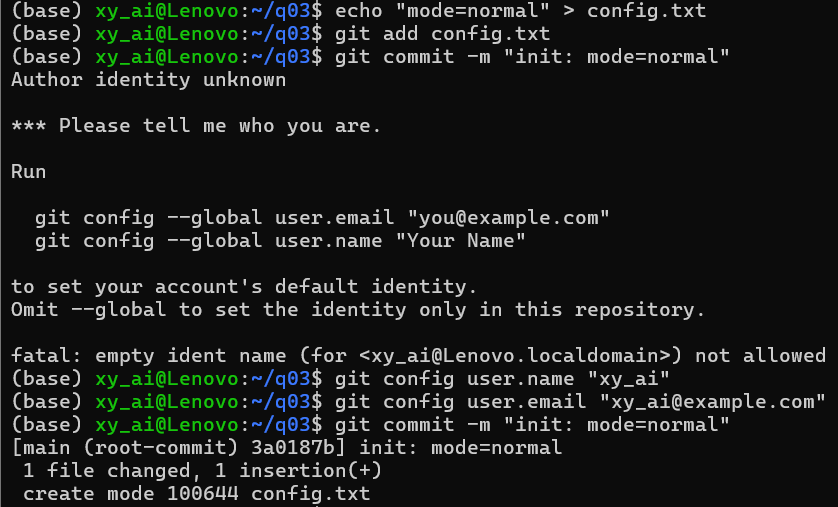
\includegraphics[width=0.85\textwidth]{36.png}
        \captionof{figure}{第一次没有输入名字和邮箱，后改进}
    \end{center}
    \item {\large 创建 feature‑a 分支，修改为mode=safe提交}
    \begin{center}
        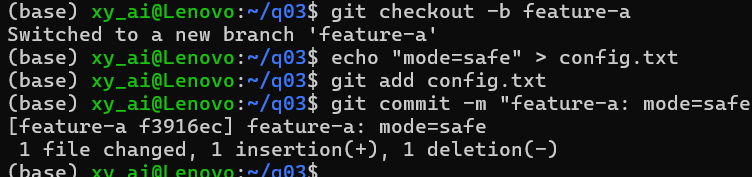
\includegraphics[width=0.85\textwidth]{37.png}
        \captionof{figure}{}
    \end{center}
    \item {\large 切回初始 main，从原始 main 创建 feature‑b 分支，修改mode=fast提交}
    \begin{center}
        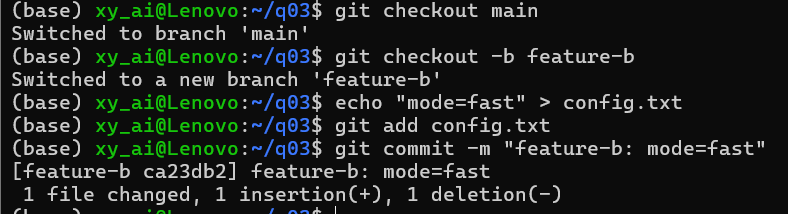
\includegraphics[width=0.85\textwidth]{38.png}
        \captionof{figure}{}
    \end{center}
    \item {\large 切回 main，先合并 feature‑a，这一步没有冲突，main 现在 config.txt 内容是mode=safe}
    \begin{center}
        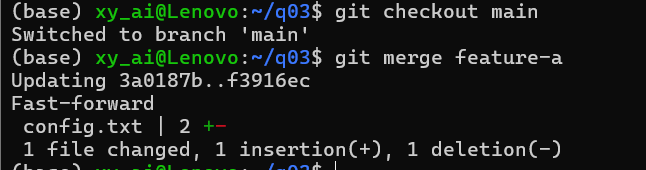
\includegraphics[width=0.85\textwidth]{39.png}
        \captionof{figure}{}
    \end{center}
    \item {\large 继续合并 feature‑b，触发合并冲突}
    \begin{center}
        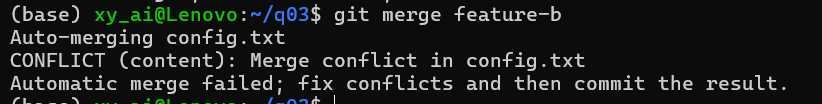
\includegraphics[width=0.85\textwidth]{40.png}
        \captionof{figure}{}
    \end{center}
    \item {\large 解决冲突，保留 mode=safe，额外增加一行 note=reviewed}
    \begin{center}
        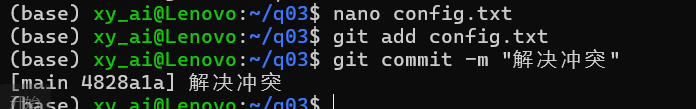
\includegraphics[width=0.85\textwidth]{41.png}
        \par\vspace{4pt}
        \captionof{figure}{冲突解决，提交合并结果}
        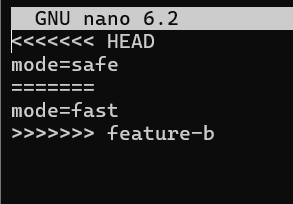
\includegraphics{42.png}
        \par\vspace{4pt}
        \captionof{figure}{按照题意改变txt之前}
        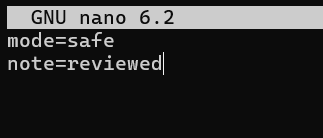
\includegraphics{43.png}
        \par\vspace{4pt}
        \captionof{figure}{按照题意改变txt之后}
    \end{center}
    \item {\large 确认工作区干净，按要求运行代码查看图形化提交日志}
    \begin{center}
        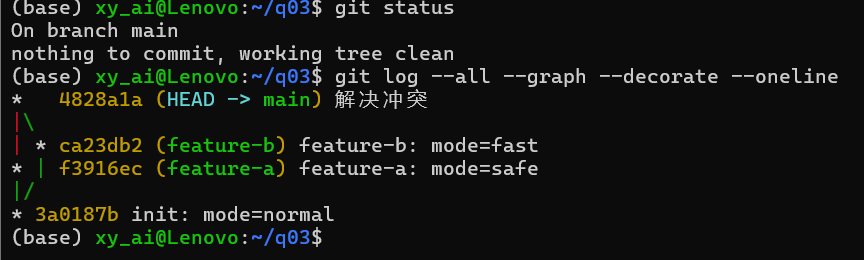
\includegraphics[width=0.85\textwidth]{44.png}
        \captionof{figure}{}
    \end{center}
\end{enumerate}

\section{第 4 题 修复并构建一页技术说明}
\begin{center}
    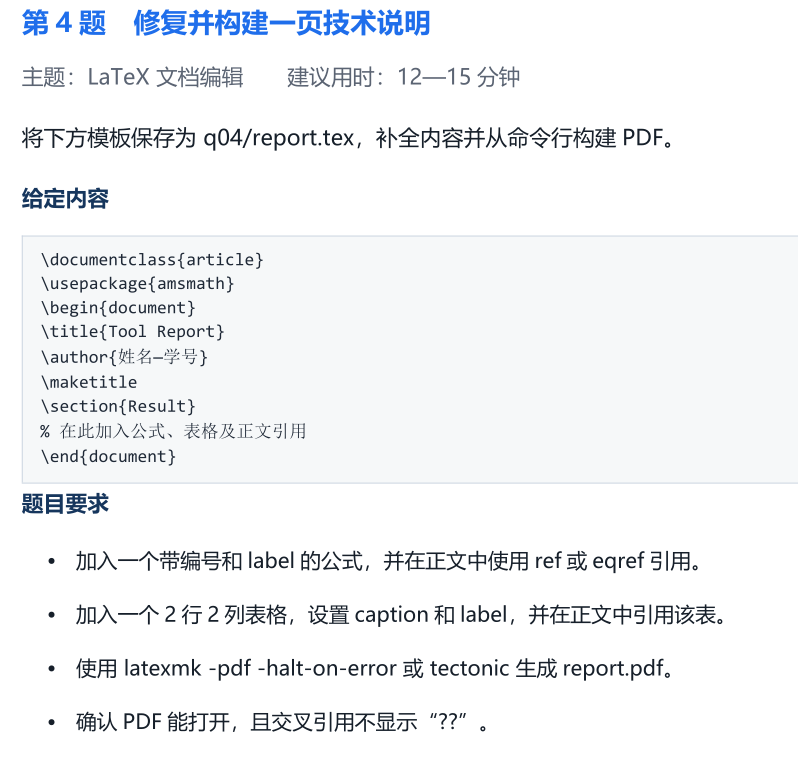
\includegraphics[width=0.86\textwidth]{24.png}
\end{center}
\begin{enumerate}
    \item {\large 创建 q04 文件夹，进入目录}
    \begin{center}
        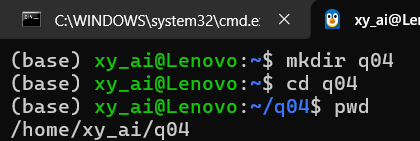
\includegraphics[width=0.88\textwidth]{25.png}
        \captionof{figure}{}
    \end{center}
    \item {\large 在wsl2中下载LaTeX}
    \begin{center}
        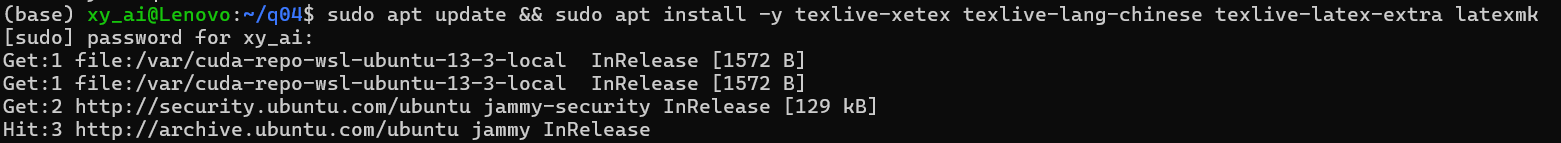
\includegraphics[width=0.88\textwidth]{26.png}
        \captionof{figure}{}
        \par\vspace{4pt}
        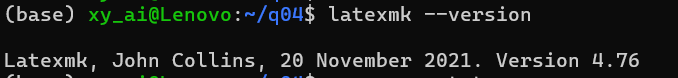
\includegraphics[width=0.83\textwidth]{27.png}
        \captionof{figure}{验证下载成功}
    \end{center}
    \item {\large 创建符合要求的 report.tex}
    \begin{center}
        
\includegraphics[width=0.88\textwidth]{28.png}
        \captionof{figure}{}
    \end{center}
    \par\vspace{4pt}
    开始编写符合要求的tex内容，包含一个带编号和 label 的公式$E = mc^2$,还有一个 2 行 2 列表格，设置 caption 和 label，均在正文按要求引用。
    \begin{center}
        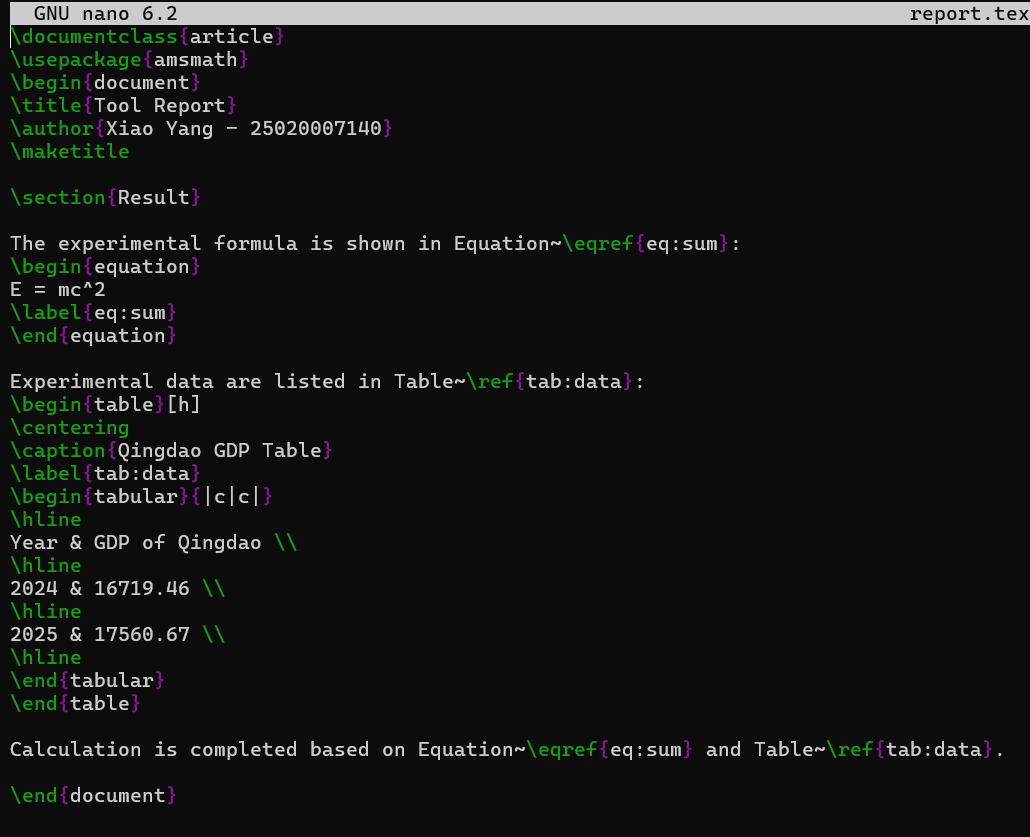
\includegraphics[width=0.83\textwidth]{29.png}
        \captionof{figure}{}
        \par\vspace{4pt}
        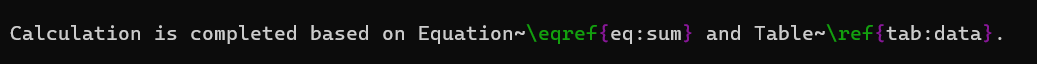
\includegraphics[width=0.83\textwidth]{33.png}
        \captionof{figure}{满足在正文引用的要求}
    \end{center}
    \item {\large 使用 latexmk -pdf -halt-on-error生成report.pdf}
    \begin{center}
        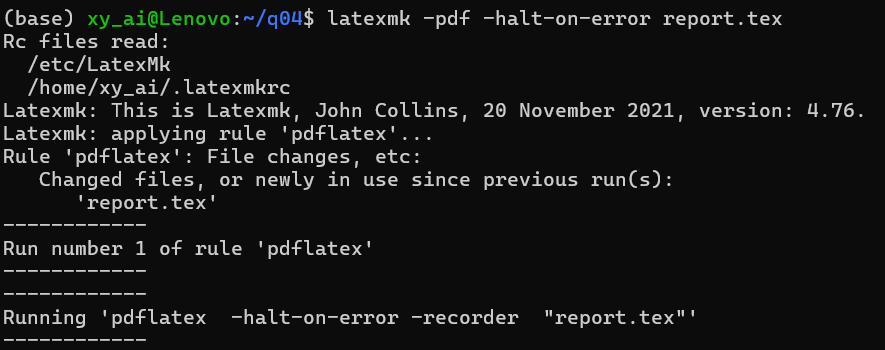
\includegraphics[width=0.88\textwidth]{30.png}
        \captionof{figure}{}
        \par\vspace{4pt}
        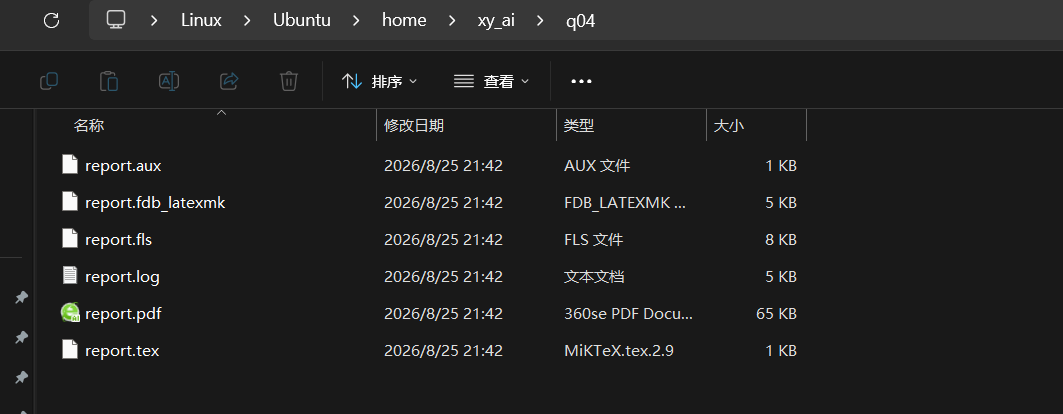
\includegraphics[width=0.83\textwidth]{32.png}
        \captionof{figure}{确认生成pdf}
    \end{center}
    \item {\large 确认 PDF 能打开，且交叉引用不显示“??”}
    \begin{center}
        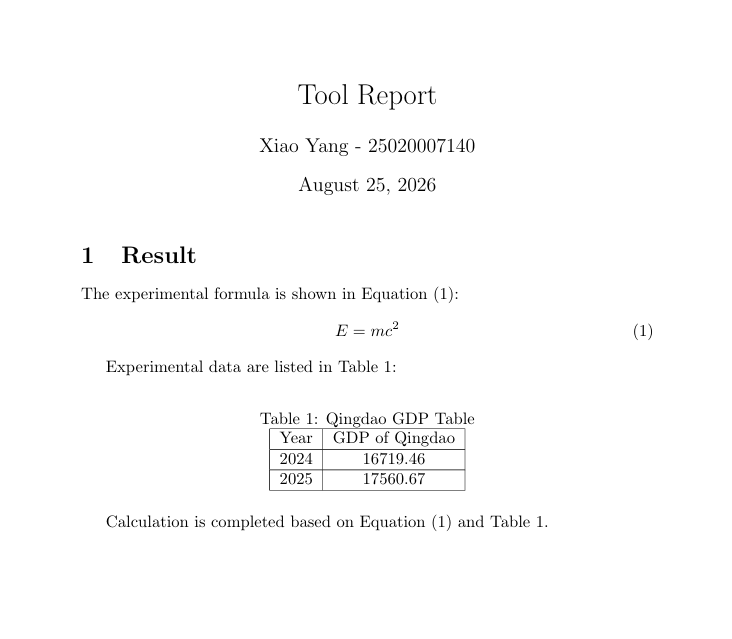
\includegraphics[width=0.88\textwidth]{31.png}
        \captionof{figure}{}
    \end{center}
\end{enumerate}




\color{red}\chapter{课后练习部分}
\color{black}


\section{课后第1题}
\begin{center}
    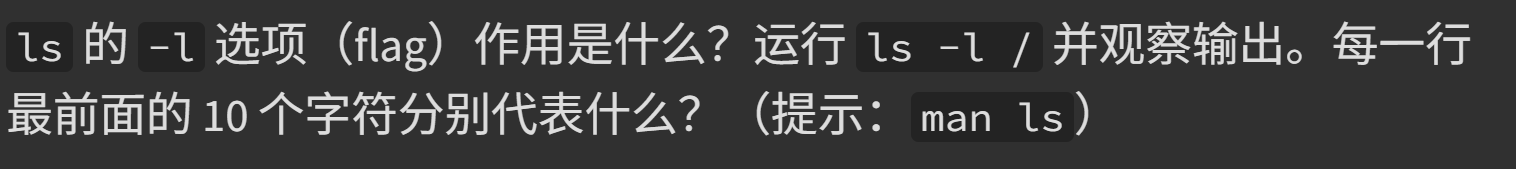
\includegraphics[width=0.88\textwidth]{45.png}
\end{center}
\begin{enumerate}
    \item {\large 运行要求代码并观察输出}
    \begin{center}
        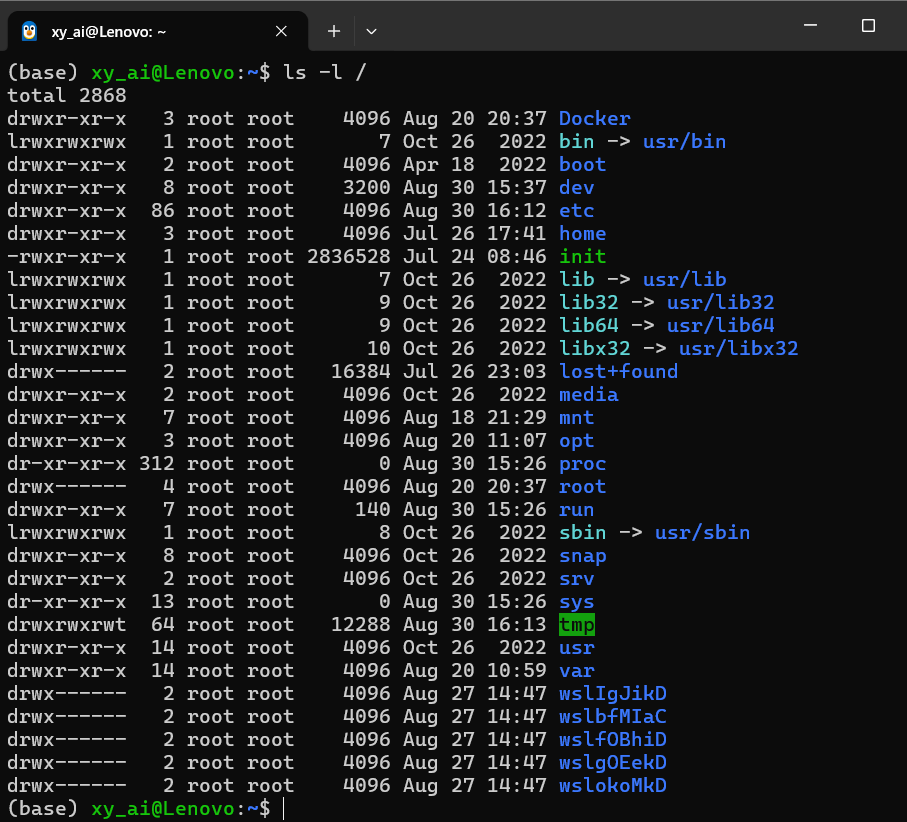
\includegraphics[width=0.88\textwidth]{46.png}
        \captionof{figure}{}
    \end{center}
    \item {\large 回答问题：\\ls命令的-l选项用于以长列表格式展示文件的详细信息。输出结果每行开头的10个字符用来描述文件类型与权限，其中第一位代表文件类型，\texttt{-}代表普通文件，\texttt{d}代表目录，\texttt{l}代表软链接，\texttt{b}代表块设备，\texttt{c}代表字符设备；第2至4位是文件属主也就是所有者的权限，分别对应读、写、执行三种权限；第5至7位是文件所属用户组的权限；第8至10位代表系统中其他所有用户的权限，\texttt{r}代表可读，\texttt{w}代表可写，\texttt{x}代表可执行，通过这三段权限位，就定义了三类不同身份用户对该文件拥有的访问能力。}
\end{enumerate}\

\section{课后第2题}
\begin{flushleft}
    {\large 问题如下：\\在脚本的 set 选项（flag）里加入 -x 会发生什么？写个简单脚本试试并观察输出。}
\end{flushleft}
\begin{enumerate}
    \item {\large 对比：不加入 -x 版本}
    \begin{center}
        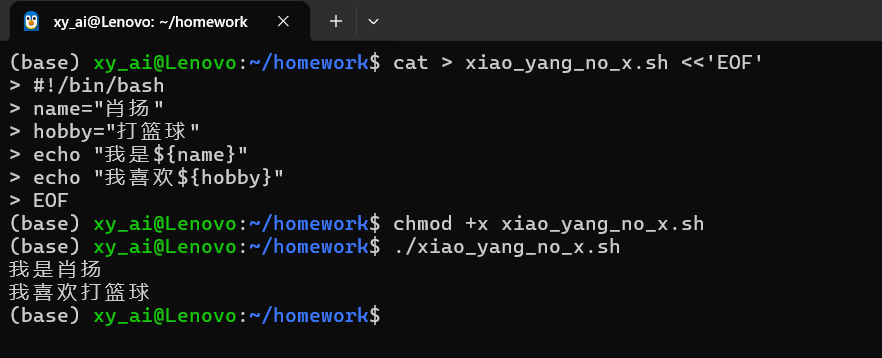
\includegraphics[width=0.88\textwidth]{47.png}
        \captionof{figure}{}
    \end{center}
    \item {\large 对比：加入 -x 版本}
    \begin{center}
        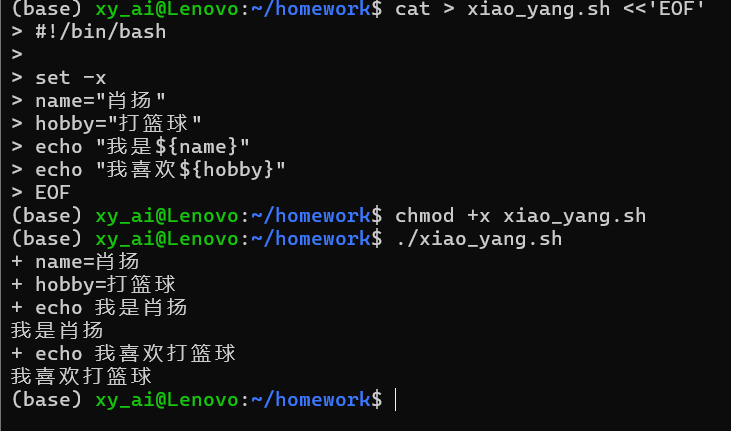
\includegraphics[width=0.88\textwidth]{48.png}
        \captionof{figure}{}
    \end{center}
    \item {\large 学到的内容：\\ set -x 是 bash 脚本的调试选项，开启后 shell 会在执行每条命令前，输出经过变量、参数展开后的实际命令，输出行以加号 + 作为标记，方便我们观察脚本真实执行的内容；没有 set -x 时脚本只会输出 echo 等命令打印的结果，看不到变量赋值这类内部执行流程}
\end{enumerate}

\section{课后第3题}
\begin{flushleft}
    {\large 问题如下：\\写一条命令，把文件复制为带当天日期的备份文件名，例如 notes.txt变为notes\_2026-01-12.txt}
\end{flushleft}
\begin{enumerate}
    \item {\large 先创建测试文件,再复制，查看文件}
    \begin{center}
        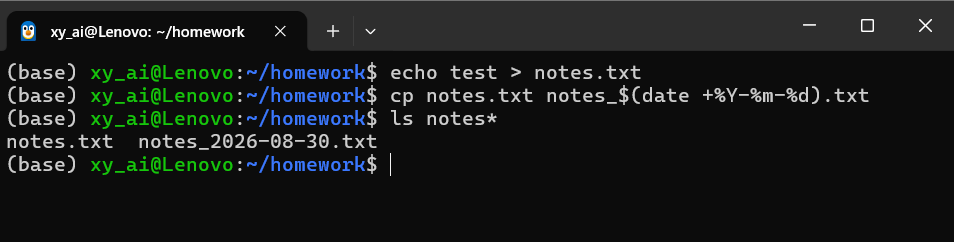
\includegraphics[width=0.88\textwidth]{49.png}
        \captionof{figure}{}
    \end{center}
\end{enumerate}

\section{课后第4题}
\begin{flushleft}
    {\large 题目如下：\\写一个脚本，接收文件名参数（\$1），用 test -f 或 [-f ...] 检查该文件是否存在，并根据结果输出不同提示。}
\end{flushleft}
\begin{enumerate}
    \item {\large 创建脚本：nano checkfile.sh}
    \begin{center}
        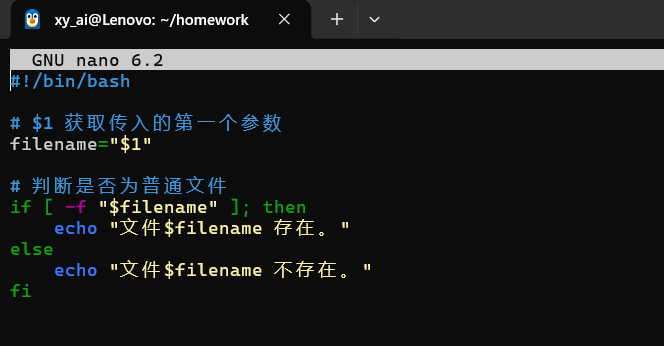
\includegraphics[width=0.88\textwidth]{65.png}
        \captionof{figure}{}
    \end{center}
    \item {\large 添加权限，测试存在和不存在的文件，检查输出结果}
    \begin{center}
        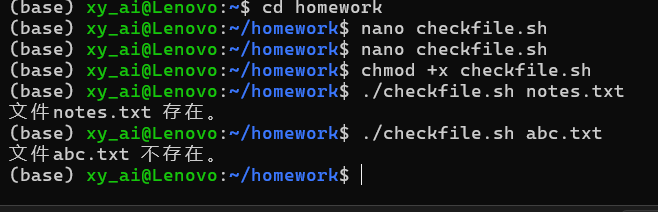
\includegraphics[width=0.88\textwidth]{66.png}
        \captionof{figure}{}
    \end{center}
\end{enumerate}\

\section{课后第5题}
\begin{flushleft}
    {\large 使用管道找出你「home 目录」中最常见的 5 种文件扩展名。（提示：组合find 、grep / sed / awk、sort、uniq -c 以及 head）}
\end{flushleft}
\begin{enumerate}
    \item {\large 如下：}
    \begin{center}
        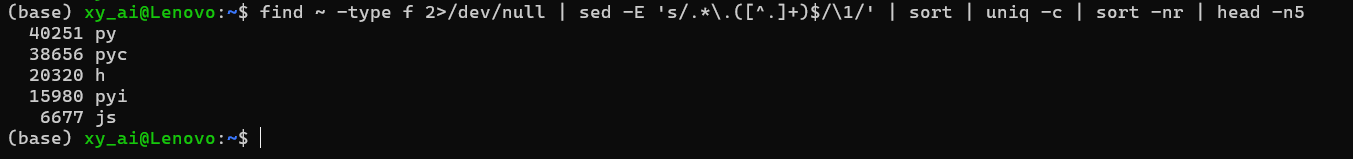
\includegraphics[width=0.88\textwidth]{67.png}
        \captionof{figure}{}
    \end{center}
\end{enumerate}


\section{课后第6题}
{\large 问题如下：克隆这门课程网站对应的代码仓库}\\
包含三个小问题：\\
1. 将版本历史以图形的形式可视化，浏览版本提交历史。\\
2. 最后一个修改 README.md 文件的人是谁？（提示：给 git log 加上参数）\\
3. \_config.yml 文件中 collections:这一行，最后一次修改对应的提交信息是什么？（提示：使用 git blame 和 git show）
\begin{enumerate}
    \item {\large 克隆库后进入}
    \begin{center}
        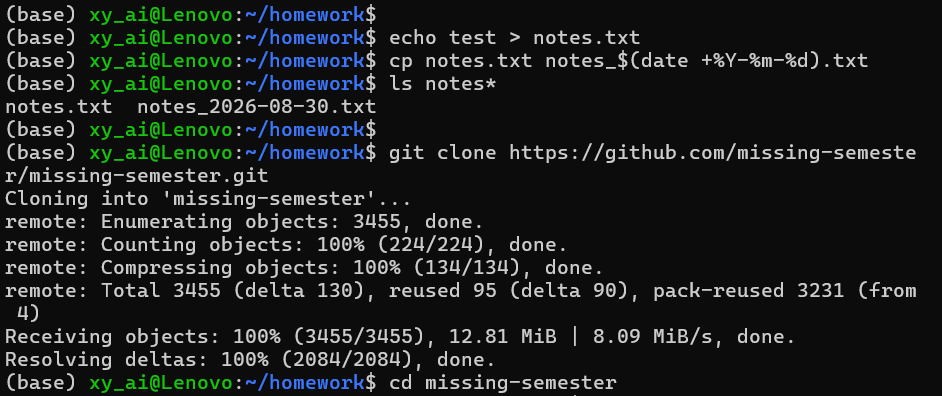
\includegraphics[width=0.88\textwidth]{50.png}
        \captionof{figure}{}
    \end{center}
    \item {\large 将版本历史可视化图形展示}
    \begin{center}
        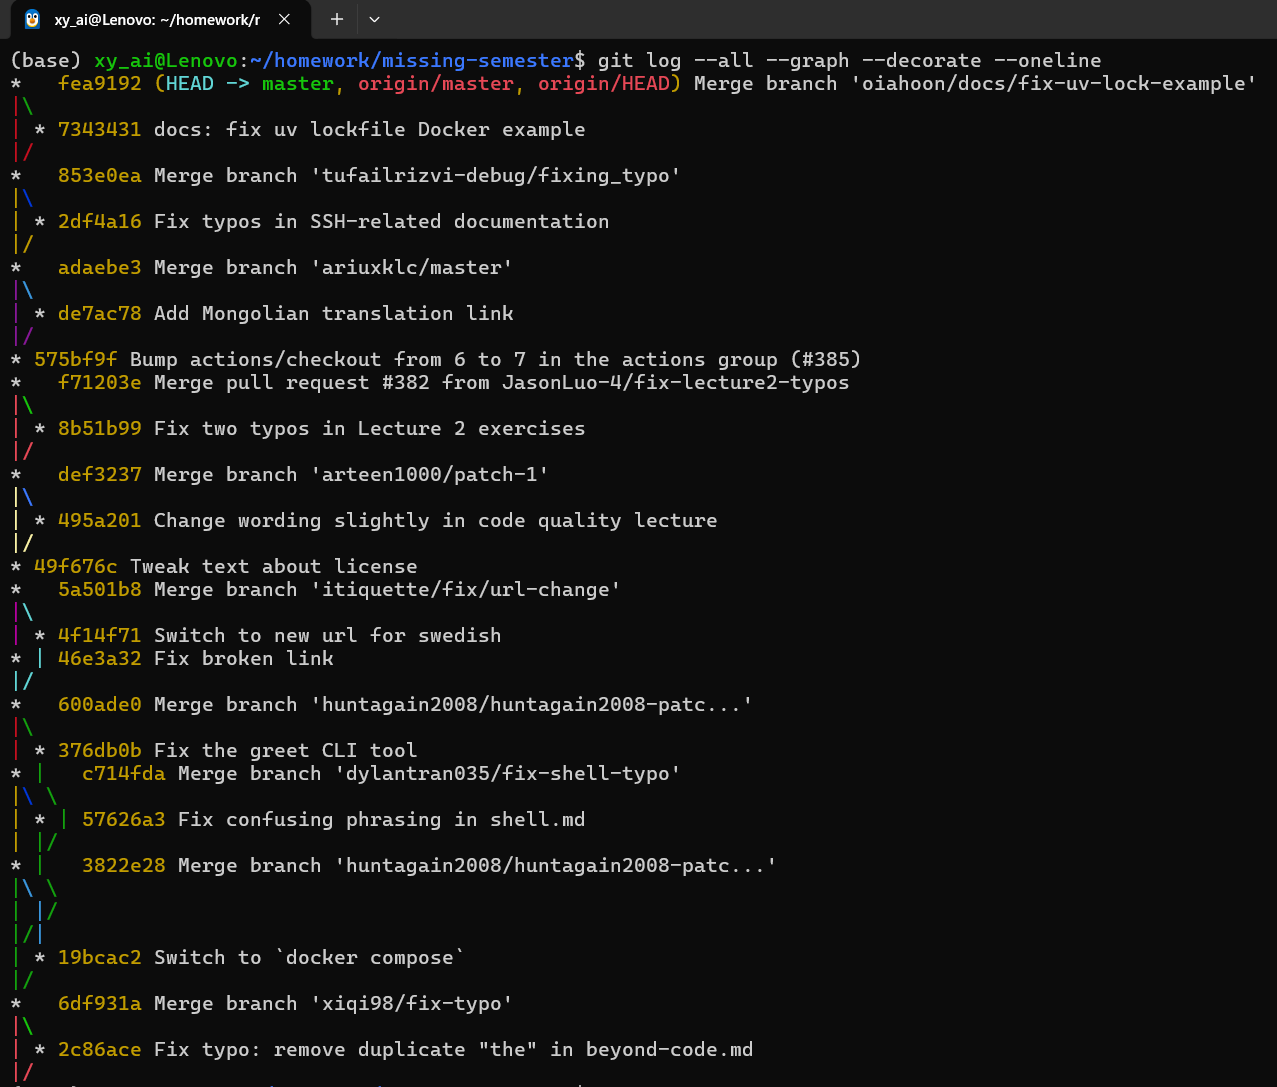
\includegraphics[width=0.88\textwidth]{51.png}
        \captionof{figure}{}
    \end{center}
    \item {\large 查询最后修改 README.md 的人}
    \begin{center}
        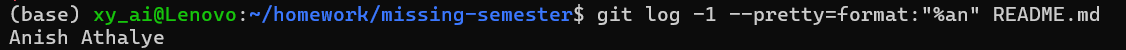
\includegraphics[width=0.88\textwidth]{52.png}
        \captionof{figure}{}
    \end{center}
    \item {\large git blame，定位这一行的 commit 哈希，然后git show，查看该提交完整信息}
    \begin{center}
        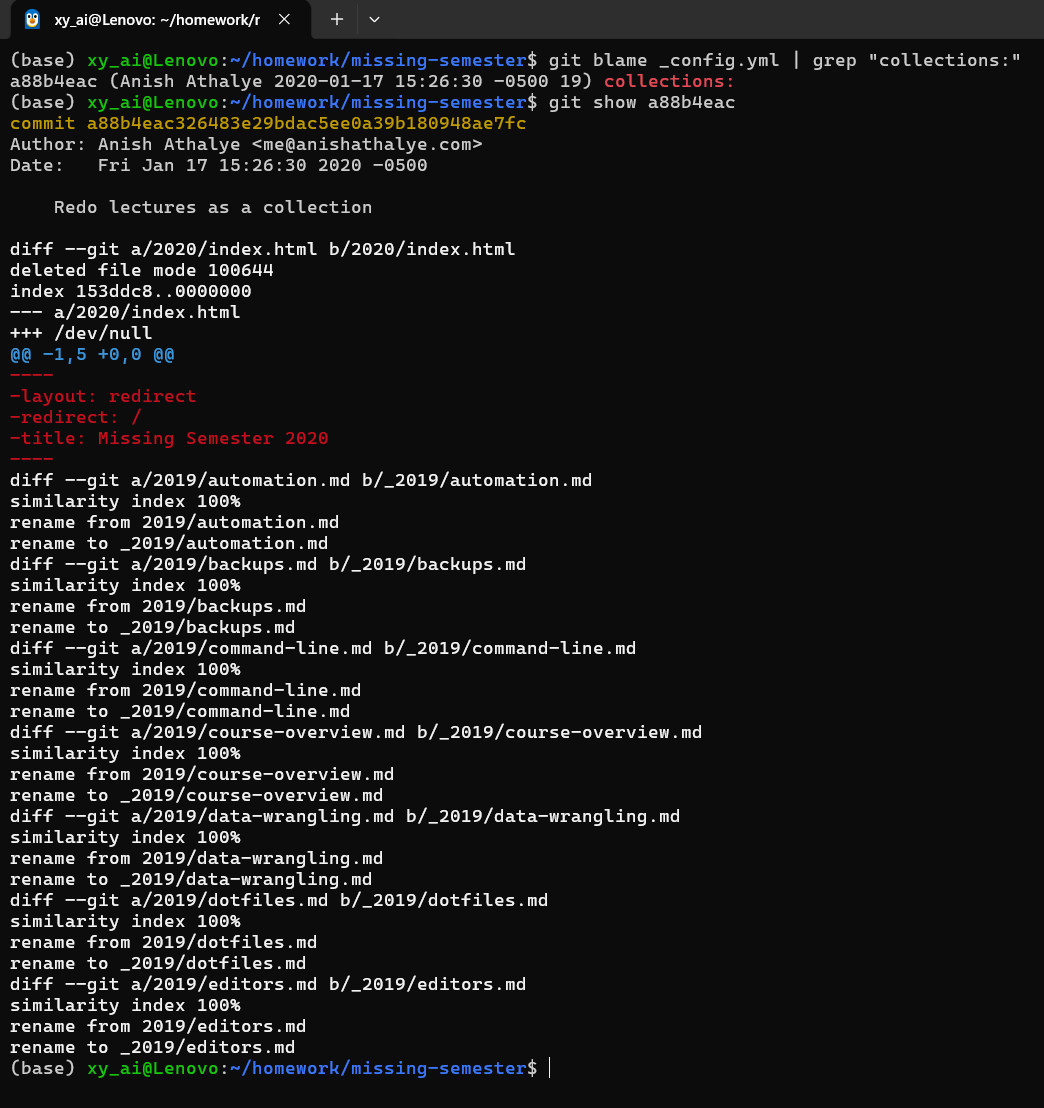
\includegraphics[width=0.88\textwidth]{53.png}
        \captionof{figure}{}
    \end{center}
\end{enumerate}

\section{课后第7题}
\begin{center}
    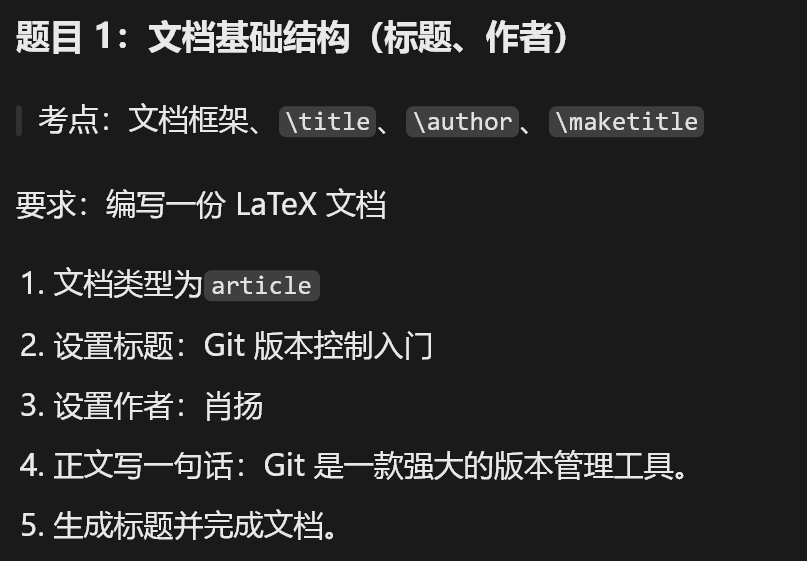
\includegraphics[width=0.88\textwidth]{54.png}
\end{center}
\begin{enumerate}
    \item {\large LaTeX代码和展示PDF如下：}
    \begin{center}
        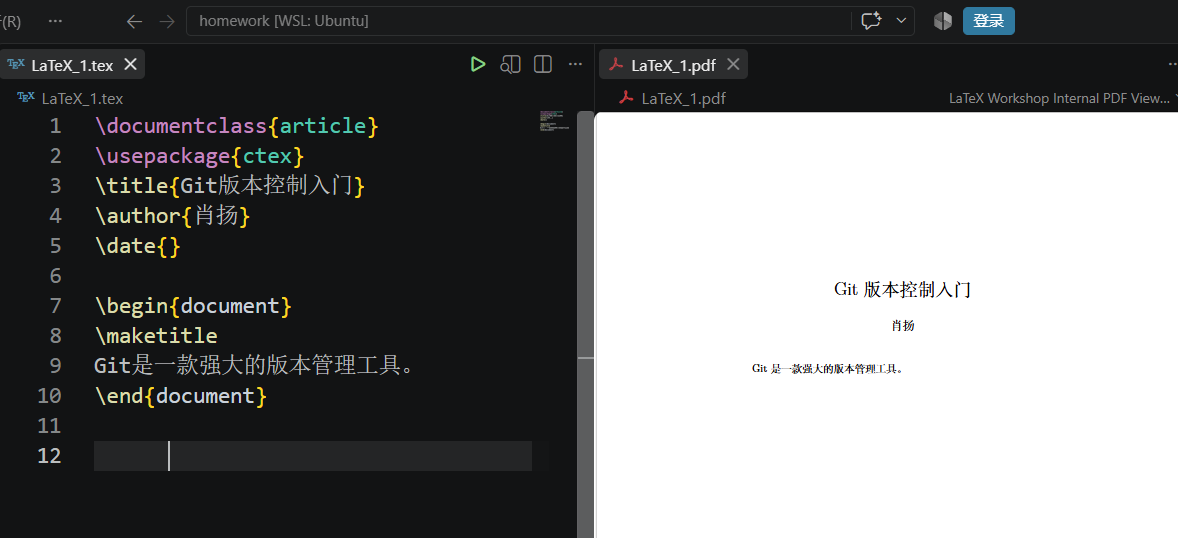
\includegraphics[width=0.88\textwidth]{55.png}
        \captionof{figure}{}
    \end{center}
\end{enumerate}

\section{课后第8题}
\begin{center}
    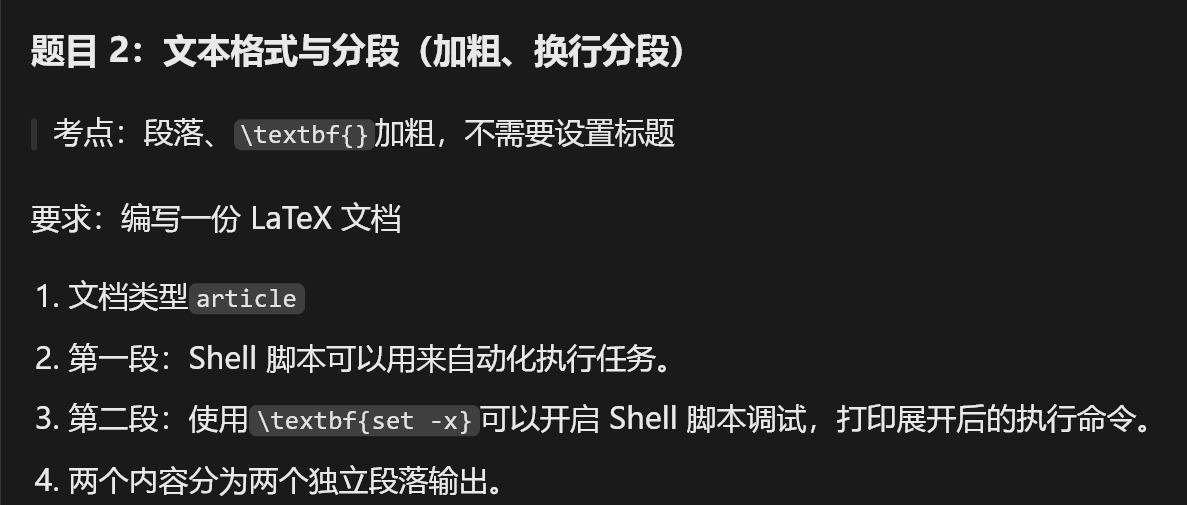
\includegraphics[width=0.88\textwidth]{56.png}
\end{center}
\begin{enumerate}
    \item {\large LaTeX代码如下：}
    \begin{center}
        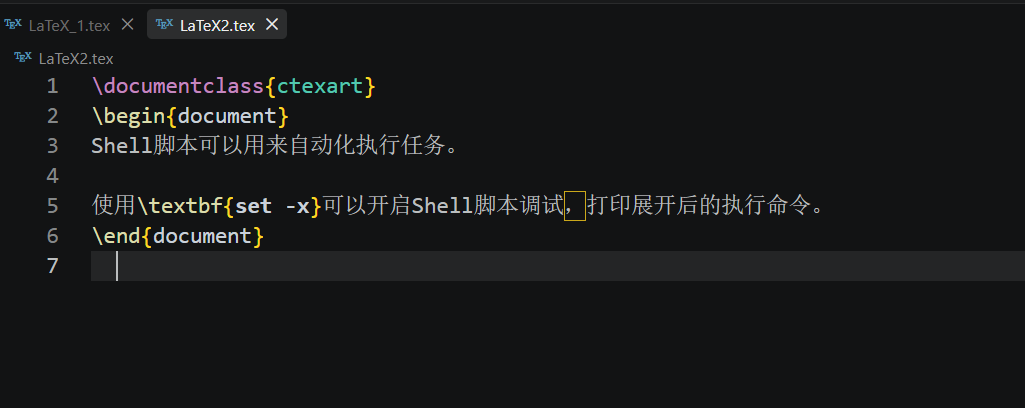
\includegraphics[width=0.88\textwidth]{57.png}
        \captionof{figure}{}  
    \end{center}
    \item {\large 呈现的PDF如下：}
    \begin{center}
        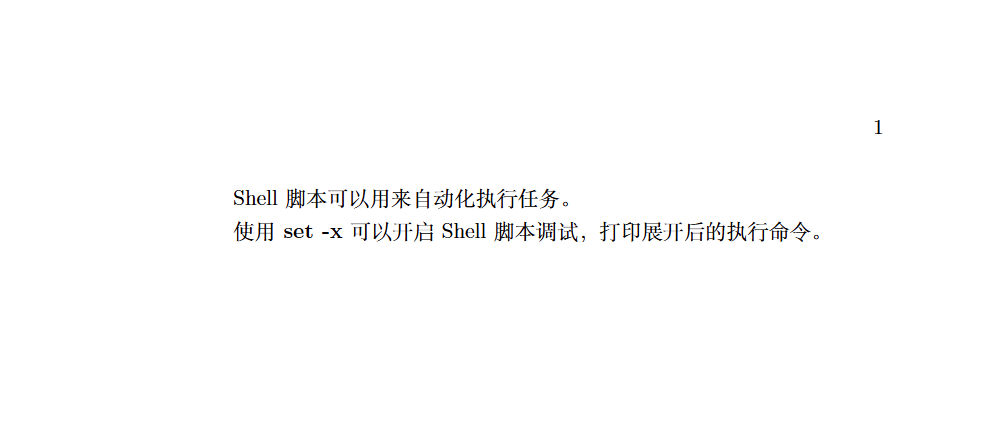
\includegraphics[width=0.88\textwidth]{58.png}
        \captionof{figure}{}  
    \end{center}
\end{enumerate}

\section{课后第9题}
\begin{center}
    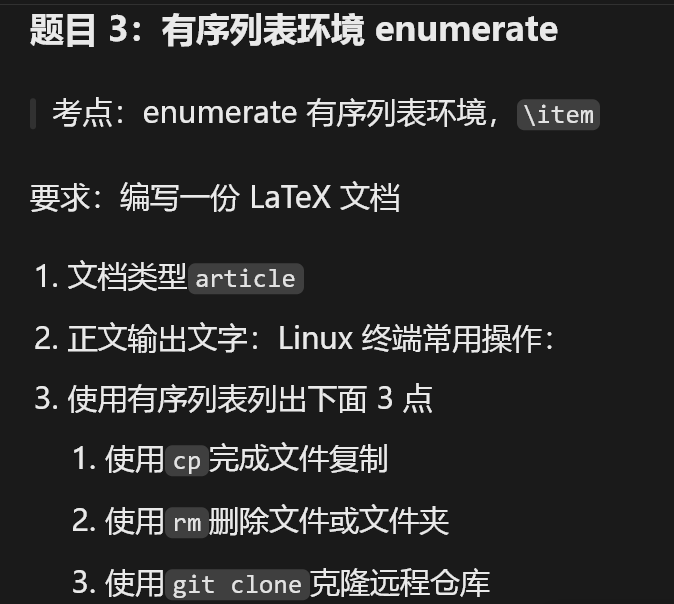
\includegraphics[width=0.88\textwidth]{59.png}
\end{center}
\begin{enumerate}
    \item {\large LaTeX代码如下：}
    \begin{center}
        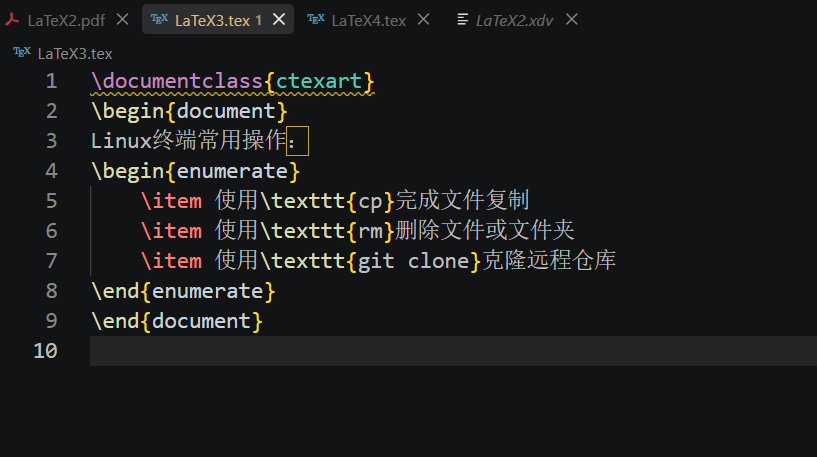
\includegraphics[width=0.88\textwidth]{60.png}
        \captionof{figure}{}  
    \end{center}
    \item {\large 呈现的PDF如下：}
    \begin{center}
        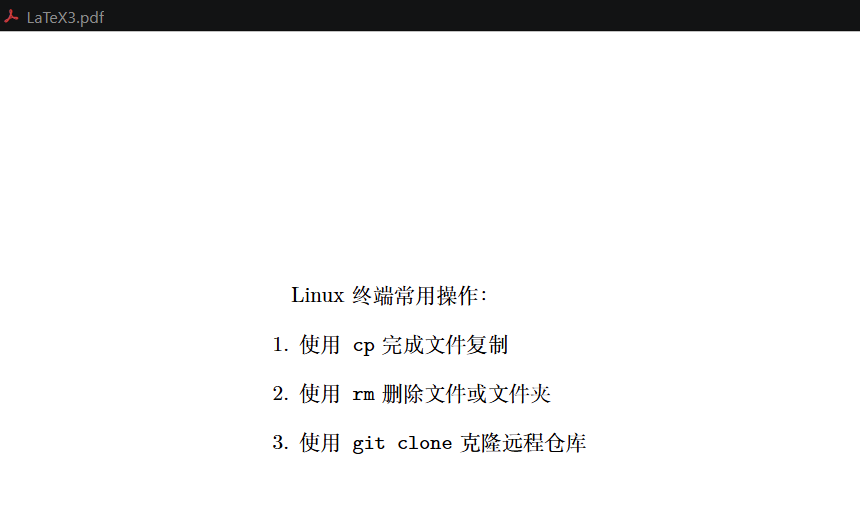
\includegraphics[width=0.88\textwidth]{61.png}
        \captionof{figure}{}  
    \end{center}
\end{enumerate}

\section{课后第10题}
\begin{center}
    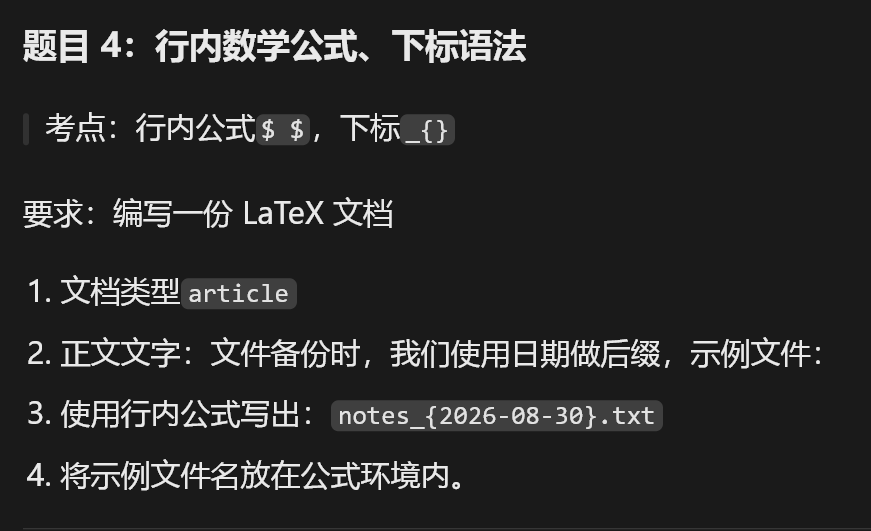
\includegraphics[width=0.88\textwidth]{62.png}
\end{center}
\begin{enumerate}
    \item {\large LaTeX代码如下：}
    \begin{center}
        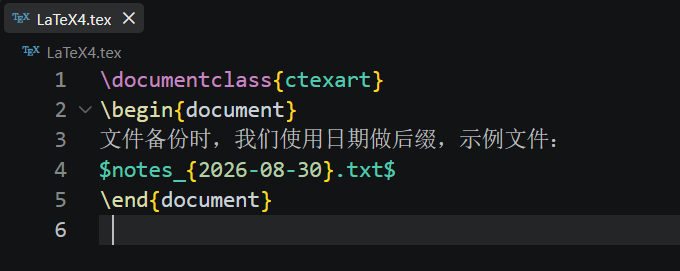
\includegraphics[width=0.88\textwidth]{63.png}
        \captionof{figure}{}  
    \end{center}
    \item {\large 呈现的PDF如下：}
    \begin{center}
        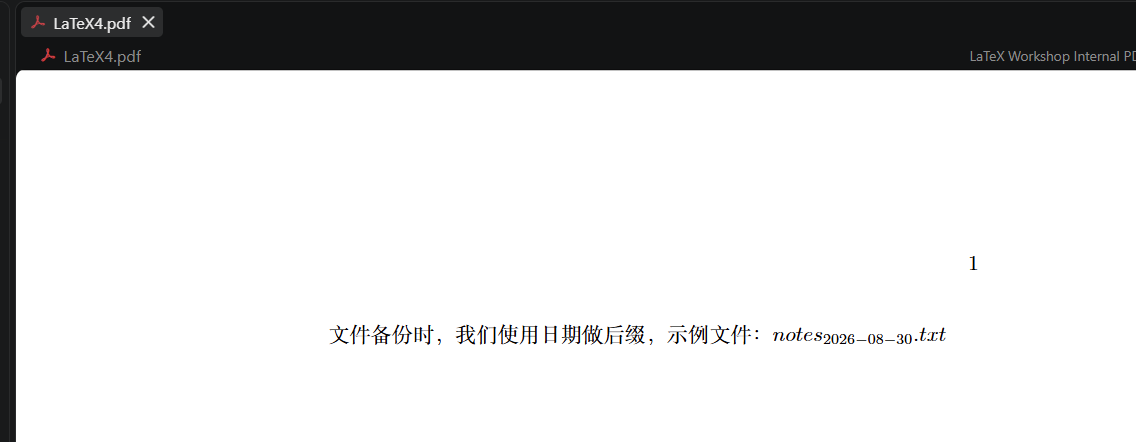
\includegraphics[width=0.88\textwidth]{64.png}
        \captionof{figure}{}  
    \end{center} 
\end{enumerate}






\color{red}\chapter{解题感悟}
\color{black}
\section{课上练习}
\begin{enumerate}
    {\large \item 解决问题1：使用LaTeX遇到无法输出汉字问题}\\
在使用LaTeX编写时，发现使用汉字会出现汉字无法输出的问题，通过写入
    \texttt{"latex-workshop.latex.recipe.default": "latexmk (xelatex)"}解决问题
    \begin{center}
        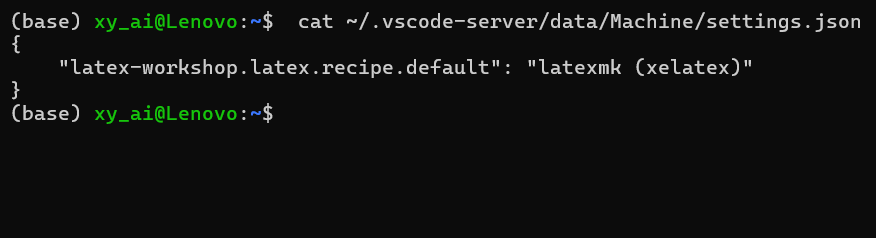
\includegraphics[width=1\textwidth]{photo1.png}
        \captionof{figure}{相关图片}
    \end{center}
    {\large \item 解决问题2：使用LaTeX遇到英文符号自动转化为中文}\\
    发现使用\texttt{"texttt"}打字机字体环境，引号不会被ctex转换，可以原样输出英文引号。
    {\large \item 解决问题3：区分ls -la input和ls -laR input}\\
    ls -la input：只看 input 这一层，不会进入 docs、tmp 子目录\\
    ls -laR input：递归往下钻，把子文件夹内部所有文件全部列出来，截图里就打印出 input/docs、input/tmp 下面的文件了，包括隐藏文件 .secret.txt。
    {\large \item 在文件整理任务中，我学会了使用 find 查找指定类型的文件，并结合 cpio 在复制文件时保留原有的目录结构。同时，我进一步理解了目录权限和普通文件权限的区别，以及 750、640 等数字权限所代表的实际含义。通过比较 ls -la input 和 ls -laR input，我也认识到普通查看与递归查看之间的区别。}
    {\large \item 在日志统计任务中，我体会到了 Shell 管道的作用。将 awk、sort、head 等工具组合起来，可以完成筛选、统计、排序和输出等一系列操作。相比手工统计，这种方法效率更高，也更适合处理大量数据。脚本对文件是否存在进行判断，并通过标准错误和非零退出码报告异常，也让我认识到一个完整的脚本不仅要能够得到正确结果，还应当具备基本的错误处理能力。}
    {\large \item Git 合并冲突练习让我理解了分支之间产生冲突的原因。当两个分支修改同一位置时，Git 无法自动判断应当保留哪一项内容，需要开发者检查冲突标记、确定最终内容并重新提交。这次练习使我不再把合并冲突简单地看成报错，而是把它理解为多人协作过程中需要人工作出选择的一种正常情况。}
    {\large \item 在 LaTeX 练习中，我掌握了公式、表格、标题和交叉引用的基本写法，也认识到 LaTeX 文档通常需要经过完整编译才能正确生成引用结果。课堂内容涵盖了文件管理、数据处理、版本控制和文档构建等多个方面，使我认识到这些工具虽然用途不同，但都强调操作规范、过程可验证和结果可复现。}

\end{enumerate}


\section{课后练习}
\begin{enumerate}
    \item {\large 在完成文件检查脚本时，脚本文件已经创建并写入了正确内容，但直接运行时出现了“Permission denied”的提示。检查后发现，脚本只有读写权限，没有执行权限。使用 chmod +x checkfile.sh 为脚本增加执行权限后，再通过 ./checkfile.sh 文件名 运行，脚本便能够正常执行。这个问题让我认识到，脚本内容正确并不代表一定能够直接运行，还需要检查文件权限。}
    \item {\large 在测试文件存在性检查时，如果文件名中带有空格，直接使用未加引号的 $1，Shell 可能会把文件名拆分成多个参数，从而造成判断失败或产生语法错误。解决方法是在条件判断和相关命令中使用双引号保护变量，例如写成 [ -f "$1" ]。修改后，即使文件名中包含空格，脚本也能把它作为一个完整路径处理。通过这个问题，我进一步理解了 Shell 脚本中为变量添加引号的重要性。}
    \item {\large 在查询 \_config.yml 中 collections: 这一行的最后修改记录时，最初只查看普通的 git log，得到的是整个仓库的提交历史，无法直接判断具体是哪一次提交修改了这一行。后来先使用 git blame \_config.yml 定位该行对应的提交哈希，再使用 git show 提交哈希 查看提交作者、时间、说明和修改内容，最终找到了需要的信息。这个问题让我明白，不同 Git 命令解决的问题不同：git log 用于查看历史，git blame 用于追踪具体代码行，git show 用于查看某次提交的详细内容。}
    \item {\large 课后练习心得总结如下：课后练习进一步巩固了课堂知识，并让我有机会独立完成更加具体的操作。通过分析 ls -l 输出，我能够根据开头的字符判断文件类型，并分别识别文件所有者、用户组和其他用户的读、写、执行权限。通过对比是否启用 set -x，我了解到它可以显示脚本中经过变量和参数展开后实际执行的命令，因此在排查脚本问题时非常有帮助。日期备份、文件存在性检查和常见扩展名统计等练习，使我更加熟悉变量、条件判断和管道组合的使用。尤其是在统计文件扩展名时，需要把多个功能单一的命令连接起来，才能完成查找、提取、排序和计数。这让我体会到 Linux 命令行的特点不是依赖某一个复杂命令，而是通过组合多个简单工具来解决问题。Git 课后练习让我学会了从不同角度查看仓库历史。git log 适合查看整体提交记录，git log -- README.md 可以查找与指定文件有关的提交，而 git blame 可以定位某一行最后由哪个提交修改，再通过 git show 查看该提交的详细信息。后面的 LaTeX 练习则进一步加深了我对文档结构、公式、表格和排版效果之间关系的理解。总体来看，课后练习提高了我独立分析问题的能力。完成任务时不能只照着命令输入，还要观察运行结果、理解命令参数，并在出现异常时逐步定位原因。只有真正理解每一步的作用，才能在题目条件发生变化时灵活调整解决方法。}
\end{enumerate}

\color{red}\chapter{上传GitHub}
\color{black}
\section{编写.gitignore}
在把课程作业上传到 GitHub 之前，我对文件夹做了清理，并在仓库根目录写入了
如下 \texttt{.gitignore}：

\begin{lstlisting}
LaTeX 编译中间产物
*.aux
*.fdb_latexmk
*.fls
*.log
*.synctex.gz
*.xdv
*.toc

Windows 下载标记
*Zone.Identifier*

个人 IDE 配置
.vscode/
\end{lstlisting}

逐条说明如下：

\begin{itemize}
    \item \texttt{*.aux}：交叉引用辅助文件，每次编译自动生成；
    \item \texttt{*.fdb\_latexmk}、\texttt{*.fls}：latexmk 记录的依赖关系和
    文件清单，属于工具内部数据；
    \item \texttt{*.log}：编译日志，只用于排查错误；
    \item \texttt{*.synctex.gz}：TeX 源码与 PDF 之间双向定位的压缩文件；
    \item \texttt{*.xdv}：xelatex 生成的中间格式，在产出 PDF 前需要先经过它；
    \item \texttt{*.toc}：目录数据文件，由 \texttt{\textbackslash tableofcontents}
    生成；
    \item \texttt{*Zone.Identifier*}：Windows 的"下载来源"标记。文件从 Windows
    复制进 WSL 时，NTFS 备用数据流会被拆成独立的
    \texttt{xxx:Zone.Identifier} 小文件（清理时共发现 324 个），写进规则后
    以后不会再混入仓库；
    \item \texttt{.vscode/}：VS Code 的个人工作区配置，不属于作业交付内容。
\end{itemize}

\section{GitHub仓库链接}
作业仓库地址（公开，默认分支 main）：

\begin{center}
{\url{https://github.com/xiaoyang1088/system_development_tools}}
\end{center}
说明：仓库名为 \texttt{system\_development\_tools}，GitHub 用户名 \texttt{xiaoyang1088}。仓库内按
题目组织为 \texttt{homework/}、\texttt{q01/} 至 \texttt{q04/}、
\texttt{实验报告/} 等目录，根目录含 \texttt{.gitignore}。

\section{commit提交记录}
\begin{center}
    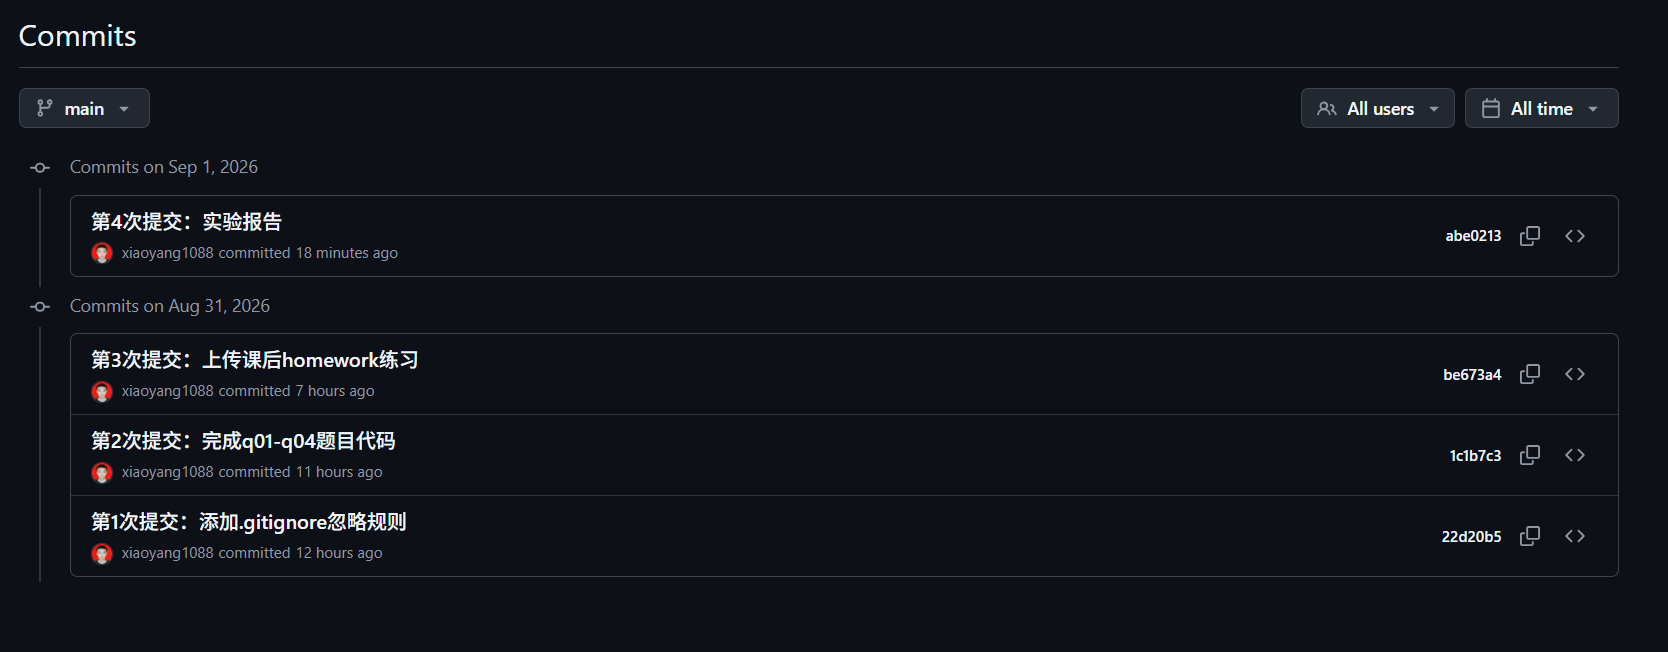
\includegraphics[width=0.88\textwidth]{200.png}
    \captionof{figure}{}
\end{center}




\end{document}